\documentclass[]{article}

% Imported Packages
%------------------------------------------------------------------------------
\usepackage{amssymb}
\usepackage{amstext}
\usepackage{amsthm}
\usepackage{amsmath}
\usepackage[shortlabels]{enumitem}
\usepackage{fancyhdr}
\usepackage[margin=1in]{geometry}
\usepackage{graphicx}
\usepackage{extarrows}
\usepackage{setspace}
\usepackage{tabto}
\usepackage{cite}
\usepackage{etoolbox}
\usepackage{hyperref}
\patchcmd{\thebibliography}{\section*{\refname}}{}{}{}
\hypersetup{
    colorlinks=true,
    linkcolor=blue,
    filecolor=magenta,      
    urlcolor=blue,
    citecolor=blue
}
\urlstyle{same}
%------------------------------------------------------------------------------

% Header and Footer
%------------------------------------------------------------------------------
\pagestyle{plain}  
\renewcommand\headrulewidth{0.4pt}                                      
\renewcommand\footrulewidth{0.4pt}                                    
%------------------------------------------------------------------------------

% Title Details
%------------------------------------------------------------------------------
\title{Software Requirements Document}
%------------------------------------------------------------------------------

% Document
%------------------------------------------------------------------------------
\begin{document}
\author{Team 2, The Triple Grobs
        \\ Jonathan Cels (celsj)
        \\ Pesara Amarasekera (amarasep)
        \\ Rupinder Nagra (nagrar5)
}
\date{February 11th, 2021}                               


\maketitle	

\section{Introduction}
\label{sec:introduction}
% Begin Section

\subsection{Purpose \& Stakeholders}
\label{sub:purpose}
% Begin SubSection
The purpose of this document is to specify the system requirements and how the system interacts with the end user. Intended stakeholders for this document include the development team, the professor of the course, and the TAs of the course.
% End SubSection

\subsection{Scope}
\label{sub:scope}
% Begin SubSection
The software product will provide the user with an implementation of a chess game. The product aims to provide an interactive and entertaining game-play experience utilizing web programming. The user will be able to play with other users online.
% End SubSection

\subsection{Definitions, Acronyms, and Abbreviations}
\label{sub:definitions_acronyms_and_abbreviations}
% Begin SubSection
\begin{enumerate}[a)]
	\item The Software Requirements Specification (SRS) is a detailed document which describes a software system to be developed.
	\item The Web Content Accessibility Guidelines (WCAG) \cite{WCAG} are guidelines on making web content more accessible to people with disabilities.
	\item Artificial Intelligence (AI) in this document refers to a computer-controlled player.
\end{enumerate}
% End SubSection

\subsection{References}
% Begin SubSection
\label{sub:references}
\bibliographystyle{unsrt}
\bibliography{citations}
% End SubSection

\subsection{Overview}
\label{sub:overview}
% Begin SubSection
The SRS document will go into depth on the description of the product in Section 2, describing functions, characteristics, and constraints on the system. In Section 3 this document will detail different use cases of the system and illustrate a use case diagram, providing an overview of the intended product behaviour. This document will list out functional and non-functional requirements that the stakeholders aim to achieve in the final product. The functional requirements will be presented in Section 4, and non-functional requirements will be in Section 5. Finally, this document will include an overview of the different development phases and possible risks in the development process.
% End SubSection
% End Section

\section{Overall Description}
\label{sec:overall_description}
% Begin Section

This section of the SRS describes the general factors such as the functions and user characteristics that affect the product and its requirements. Also, it provides a background for these requirements to make them easier to understand.

% \subsection{Product Perspective}
% \label{sub:product_perspective}
% % Begin SubSection
% \begin{enumerate}[a)]
%     \item \href{https://github.com/techwithtim/Online-Chess-Game}{Online Chess Game} is a the baseline product we are trying to produce in this project
% 	\item The product is not self-contained as it requires interfacing with external entities for multi-player game-play.
% \end{enumerate}
% % End SubSection

\subsection{Product Functions}
\label{sub:product_functions}
% Begin SubSection
\begin{enumerate}[a)]
	\item The user can start a game with a chosen player or AI opponent. During the game users can choose to resign a game, draw a game, make a move on the board, or use the chat window to interact with the other player.
	
	\item The following are the functions explained in more detail:
	\begin{itemize}
		\item The host player is able to start the game against an AI or another user. The timer will then begin for whichever player has the current move. 
		\item Either player can choose to resign the game, terminating the game and causing their opponent to win.
		\item Either player can choose to draw the game. If this is selected, the other player must accept a draw as well. If both players accept, the game terminates and the game is a tie.
	    \item Either player can choose to make a move on the board using a drag-and-drop mechanism for a piece. The move will only be made if it is a legal move.
	    \item Either player can also interact using the chat window.
	\end{itemize} 
\end{enumerate}
% End SubSection

\subsection{Constraints}
\label{sub:constraints}
% Begin SubSection
\begin{enumerate}[a)]
	\item Time constraint: The final product must be fully implemented by the end of the semester.
	\item Resource constraint: The developers will have limited access to additional resources such as more developers, money, and software management tools.
\end{enumerate}
% End SubSection

\subsection{Facts, Assumptions, and Dependencies}
\label{sub:assumptions_and_dependencies}
% Begin SubSection
\begin{enumerate}[a)]
    \item It is assumed that the user has access to the required hardware and internet connection required to access and play the game without the hindrance of lag or other issues.
    \item It is assumed that the user has access to I/O devices, such as a keyboard/mouse/monitor for a computer, or a touchscreen for a mobile device.
	\item Based on the browser used for the web application, the  \textbf{HTML} and  \textbf{CSS} might be affected. This project will use the assumption that a user will be using the latest version of Google Chrome.
	\item It is assumed that the user has proficiency in the English language.
\end{enumerate}
% End SubSection
% End Section

\section{Use Cases}
\label{sec:use_case_diagram}
% Begin Section
This section will include a description of intended use cases, accompanied by an illustration of the use case diagram for the system.

\begin{enumerate}[{UC}1.]
    %Use case 1
    \item \textbf{Select Opponent}
        \begin{enumerate}[{ }]
            \item \textbf{Related Requirements}
                \begin{enumerate}
                    \item FR1, FR2 stated in section 4, UC1.
                    \item FR3, FR4, FR5, FR6, FR7, FR8, FR9, FR10 stated in section 4, UC2.
                    \item FR11, FR12, FR13 stated in section 4, UC3.
                \end{enumerate}
            
            \item \textbf{Initiating Actor:} 
                User

            \item \textbf{Actor's Goal:} 
                To choose between playing against an AI or a human player.
            
            \item \textbf{Participating Actors:} 
                System
            
            \item \textbf{Pre-conditions}
                The system displays the menu of available options. The choices are ``AI'' and ``Online Player''.
            
            \item \textbf{Post-conditions}
                The ``Start Game'' use case is initiated.
                
            \item \textbf{Flow of Events of Main Success Scenario:}
               \begin{enumerate}
                    \item Host player selects one of two player options, ``AI'' or ``Online Player''.
                    \item The application is initialized based on the choice made by the host. The game now starts.
                \end{enumerate}
        \end{enumerate}

    %Use case 2
    \item \textbf{Start Game}
        \begin{enumerate}[{ }]
            \item \textbf{Related Requirements}
                \begin{enumerate}
                    \item FR14, FR15, FR16, FR17, FR18 from section 4, UC4.
                \end{enumerate}
            
            \item \textbf{Initiating Actor:} 
                User

            \item \textbf{Actor's Goal:} 
                To start playing a game against the selected opponent.
            
            \item \textbf{Participating Actors:} 
                System
            
            \item \textbf{Pre-conditions}
                An ``AI`` or ``Online Player`` was selected as the opponent.
                
            \item \textbf{Post-conditions}
                The board is setup and one or two players are connected and able to play the game.
                
            \item \textbf{Flow of Events of Main Success Scenario:}
               \begin{enumerate}
                    \item Either the ``AI'' or ``Online Player'' opponent option is selected.
                    \item The server connects the two players together, or connects one player to the AI.
                    \item The board is initialized to the starting state and piece colors (black or white) are arbitrarily selected between the players.
                    \item Control is passed to the user with the white pieces and the timers are initialized.
                \end{enumerate}
        \end{enumerate}
        
    %Use case 3
    \item \textbf{Make Move}
        \begin{enumerate}[{ }]
            \item \textbf{Related Requirements}
                \begin{enumerate}
                    \item FR19, FR20, FR21, FR22, FR23, FR24, FR25 stated in section 4, UC5.
                \end{enumerate}
            
            \item \textbf{Initiating Actor:} 
                User

            \item \textbf{Actor's Goal:} 
                To make a move in the game against the opponent.
            
            \item \textbf{Participating Actors:} 
                System
            
            \item \textbf{Pre-conditions}
                The game has been started and the opponent has made their move.
                
            \item \textbf{Post-conditions}
                The game may be terminated, or the opponent is now able to make their move.
                
            \item \textbf{Flow of Events of Main Success Scenario:}
               \begin{enumerate}
                    \item The user makes a legal move.
                    \item The application registers that the user has made a move and then determines if the game must continue.
                    \item If the game has not ended, the opponent is now able to make their move.
                \end{enumerate}
                
            \item \textbf{Flow of Events for Extensions (Alternate Scenarios):}
               \begin{enumerate}
                    \item The user may make a legal move.
                    \item The application will register that the user has made a move, where it must determine if the game must continue.
                    \item If the game has not ended, the opponent is now able to make their move.
                \end{enumerate}
        \end{enumerate}

    %Use case 4
    \item \textbf{Check Legal Move}
        \begin{enumerate}[{ }]
            \item \textbf{Related Requirements}
                \begin{enumerate}
                    \item FR26, FR27, FR28 stated in section 4, UC6.
                \end{enumerate}
            
            \item \textbf{Initiating Actor:} 
                User

            \item \textbf{Actor's Goal:} 
                To determine if the move made is valid.
            
            \item \textbf{Participating Actors:} 
                System
            
            \item \textbf{Pre-conditions}
                \begin{enumerate}
                    \item The game has started.
                    \item The user has made a move.
                \end{enumerate}
                
            \item \textbf{Post-conditions}
                The game may be terminated, or the opponent is now able to make their move.
                
            \item \textbf{Flow of Events of Main Success Scenario:}
               \begin{enumerate}
                    \item The user makes a move.
                    \item The application will register that the user has made a move, where it must determine if the game must continue.
                    \item The application will check the game logic to determine if the move is legal.
                    \item If the game has not ended, the opponent is now able to make their move.
                \end{enumerate}
        \end{enumerate}
        
    %Use case 5
    \item \textbf{Initiate Chat}
        \begin{enumerate}[{ }]
            \item \textbf{Related Requirements}
                \begin{enumerate}
                    \item FR29, FR30, FR31, FR32 stated in section 4, UC7.
                \end{enumerate}
            
            \item \textbf{Initiating Actor:}
                User
                
            \item \textbf{Actor's Goal:}
                To initiate communication between players while concurrently playing a game.
                
            \item \textbf{Participating Actors:}
                System
                
            \item \textbf{Pre-conditions:}
                \begin{enumerate}
                    \item The player has started a game against another player.
                \end{enumerate}
            \item \textbf{Post-conditions:}
                \begin{enumerate}
                    \item The player has communicated with the other player.
                    \item The game-play is continued asynchronously.
                \end{enumerate}
            \item \textbf{Flow of Events of Main Success Scenario:}
                \begin{enumerate}
                    \item A game has started between two players.
                    \item One of the players selects the chat function and types a message.
                    \item The message is passed to the other player and made visible.
                    \item The opponent is able to asynchronously send messages and continue game-play.
                \end{enumerate}
        \end{enumerate}
        
    %Use Case 6
    \item \textbf{End Chat}
        \begin{enumerate}[{ }]
            \item \textbf{Related Requirements}
                \begin{enumerate}
                    \item FR33, FR34, FR35, FR36 stated in section 4, UC8.
                \end{enumerate}
            
            \item \textbf{Initiating Actor:}
                User
                
            \item \textbf{Actor's Goal:}
                To stop communicating with one's live opponent.
                
            \item \textbf{Participating Actors:}
                User
                
            \item \textbf{Pre-conditions:}
                \begin{enumerate}
                    \item The player has selected an opponent.
                    \item The player has started a game.
                \end{enumerate}
            \item \textbf{Post-conditions:}
                \begin{enumerate}
                    \item The player has made contact with the other player.
                    \item The game-play is continued asynchronously.
                \end{enumerate}
            \item \textbf{Flow of Events of Main Success Scenario:}
               \begin{enumerate}
                    \item A player initiates chat with their opponent.
                    \item One of the players can at anytime choose to end the chat session.
                    \item One player ending the chat closes the chat for both players.
                \end{enumerate}
        \end{enumerate}
        
    %Use case 7
    \item \textbf{Start Timers}
        \begin{enumerate}[{ }]
            \item \textbf{Related Requirements}
                \begin{enumerate}
                    \item FR37, FR38, FR39 stated in section 4, UC9.
                \end{enumerate}
            
            \item \textbf{Initiating Actor:} 
                System

            \item \textbf{Actor's Goal:} 
                To start the timer for each player that represents how long each player has to make their moves in the game.
            
            \item \textbf{Participating Actors:} 
                User
            
            \item \textbf{Pre-conditions}
                The game has been started and the player with the white pieces has made a move.
                
            \item \textbf{Post-conditions}
                The timers have begun to countdown from their original values.
                
            \item \textbf{Flow of Events of Main Success Scenario:}
               \begin{enumerate}
                    \item The user with the white pieces makes a legal move.
                    \item The timer for the user with the black pieces begins to count down from its initial value.
                    \item The user with the black pieces makes a legal move, or that player's timer reaches 0. 
                    \item If a legal move is made, that timer is paused and the other timer begins to count down from its initial value.
                    \item If a timer reaches 0, the ``Terminate Game'' use case occurs and is overridden by ``Timeout''.
                \end{enumerate}
        \end{enumerate}

    %Use case 8
    \item \textbf{Terminate Game}
        \begin{enumerate}[{ }]
            \item \textbf{Related Requirements}
                \begin{enumerate}
                    \item FR40 stated in section 4, UC10.
                    \item FR41 stated in section 4, UC11.
                    \item FR42 stated in section 4, UC12.
                    \item FR43 stated in section 4, UC13.
                    \item FR44 stated in section 4, UC14.
                    \item FR45 stated in section 4, UC15.
                \end{enumerate}
            
            \item \textbf{Initiating Actor:} 
                Any of: User, or System

            \item \textbf{Actor's Goal:} 
                To determine if the game must be ended.
            
            \item \textbf{Participating Actors:} 
                None
            
            \item \textbf{Pre-conditions}
                The game has been started.
                
            \item \textbf{Post-conditions}
                The game has ended with a definite result.
                
            \item \textbf{Flow of Events of Main Success Scenario:}
               \begin{enumerate}
                    \item The system must start the game.
                    \item The application determines if a user has offered a decision to end the game in a resignation or draw. The other user can choose to accept or reject this offer.
                    \item The application determines if the user has won or lost the game through checkmate, stalemate or timeout. This signifies that one of the players can no longer make any moves.
                    \item The game will end in a definite result if any of the previous events are true.
                \end{enumerate}
        \end{enumerate}
\end{enumerate}

\bigskip
Below is a visualization of the above use cases as part of a use case diagram.
\medskip

\begin{figure}[ht]
    \centering
    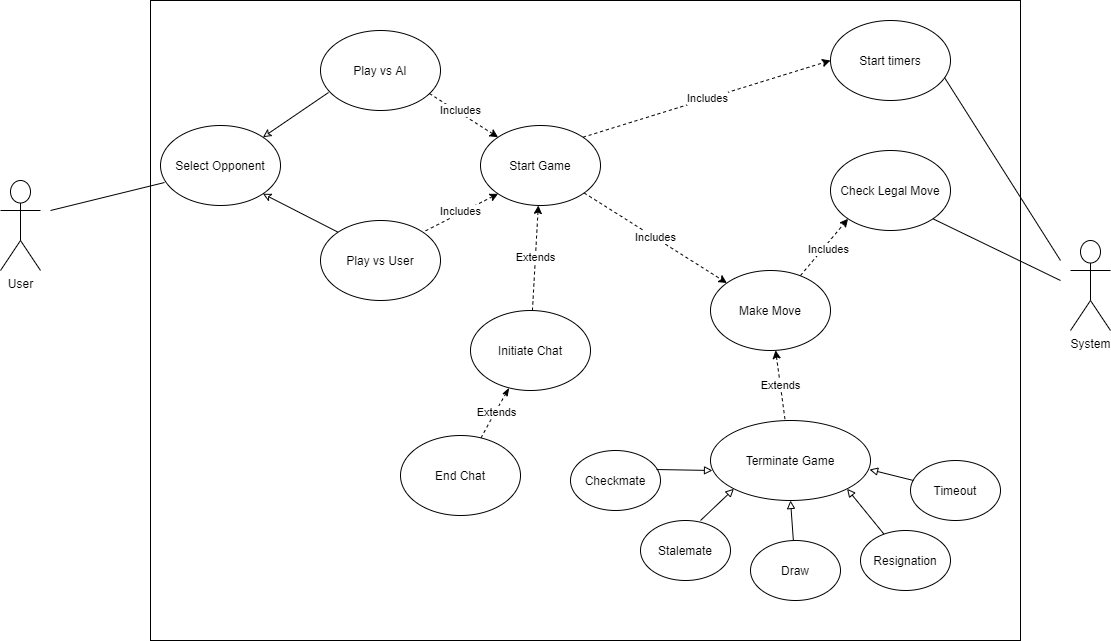
\includegraphics[width=50em,height=35em]{UseCaseDiagram.png}
    \caption{UML Use Case Diagram}
    \label{fig:usecase}
\end{figure}

\section{Functional Requirements}
\label{sec:functional_requirements}
% Begin Section
This section of the SRS contains all of the functional software requirements. The functional requirements detailed here enable designers to design a system that satisfies these requirements, and enable testers to test that the system satisfies these requirements.

\begin{enumerate}[{UC}1.]
	\item \textbf{Select Opponent}
	\begin{enumerate}[{FR}1.]
	    \item The user shall connect to the web application server.
		\item The user shall be immediately presented with the option of playing with an ``AI'' or ``Online Player'' in the middle of their screen. They shall use the labeled buttons to choose between the two options in order to proceed.
	\end{enumerate}
	
	\item \textbf{Play Against Live Opponent}
	\begin{enumerate}[{FR}1., resume]
		\item If a user decides to ``Play Against a Live Opponent'' the system shall pair them against a user with the same invite link.
		\item While the system is awaiting another player, the system shall be present the user with the options to ``Quit'', or ``Play Against AI''.
		\item If a user decides to ``Quit'' or ``Play Against AI'' the current game shall be terminated.
		\item If a user selects the ``Quit'' option, the system shall return them to the ``Select Opponent'' use case.
		\item If a user selects the ``Play Against AI'' option, the system shall send them to the ``Play Against AI'' use case.
		\item The system shall present the players with a loading screen while the application is initializing the game. The loading screen shall last no longer than 5 seconds.
		\item Once initialized, the system shall present the players with a view of the board and transfer to the ``Start Game'' use case.
		\item If a user requests to start a game on any server with 15 concurrent games, the system shall reject the request and return to the ``Select Opponent'' use case.
	\end{enumerate}
	
	\item \textbf{Play Against AI}
	\begin{enumerate}[{FR}1., resume]
		\item If a user selects ``Play Against AI'' the system shall immediately transfer to the ``Start Game'' use case.
        \item While playing against the AI the system shall have no option to initiate chat.
		\item If a user requests to start a game on any server with 15 concurrent games, the system shall reject the request and return the user to the ``Select Opponent'' use case.
	\end{enumerate}
	
	\item \textbf{Start Game}
	\begin{enumerate}[{FR}1., resume]
		\item If the user chooses ``AI'' from the ``Select Opponent'' use case, the server shall connect to an AI player and arbitrarily assign black or white to each player.
		\item If the user chooses ``Online Player'' from the ``Select Opponent'' use case, a shareable link shall be created with which a player can join the server. If a player joins, each player shall be arbitrarily assigned black or white.
		\item The board and pieces shall be initialized, and the orientation of the board will be determined based on the colour of the users pieces. 
		\item The timer shall be initialized with a countdown of 10 minutes for each player, and the game control is dependent on the player with the white pieces.
		\item The system shall give exclusive control to the player with the white pieces and start that player's timer.
	\end{enumerate}
	
	\item \textbf{Make Move}
	\begin{enumerate}[{FR}1., resume]
		\item The system shall not allow the player to make a move until their opponent has played a move, with the exception of the first move of the game.
		\item If a player clicks a piece, holds the mouse down, drags the piece to a square, and releases the mouse, the system shall register an attempted move.
		\item The application shall confirm that the move is legal as defined by the rules of the game. 
		\item If the attempted move is legal, the move shall be sent to the server and the opposite player shall be given control.
		\item If the attempted move is not legal, the move shall not be sent to the server and the player shall retain control.
		\item The `Terminate Game` use case shall be checked after every move is made.
		\item If the game is not terminated, the timer for the other player shall resume.
	\end{enumerate}
	
	\item \textbf{Check Legal Move}
	\begin{enumerate}[{FR}1., resume]
		\item The application shall register the move the user has made, and check the program logic to determine if the move can be made.
		\item The move is then reflected in the board state and the opponent may now make their move.
		\item Only one player will be allowed to make a move at once.
	\end{enumerate}
	
	\item \textbf{Initiate Chat}
	\begin{enumerate}[{FR}1., resume]
		\item The system shall present the user with an option to ``Start Chat'' to start a chat.
		\item If ``Start Chat'' is selected, the system shall open a chat window for both players.
		\item If both players click on the ``Start Chat'' button simultaneously then the system shall only register one of the selections.
		\item The ``Start Chat'' button shall be replaced by an ``End Chat'' button.
	\end{enumerate}
	
	\item \textbf{End Chat}
	\begin{enumerate}[{FR}1., resume]
		\item The system shall present the user with an option to ``End Chat'' at any time once a chat has started.
		\item If the chat is ended by one player the chat shall be disabled for both players. The ``End Chat'' button shall be replaced by the ``Start Chat'' button.
		\item If both players click on the ``End Chat'' button simultaneously then the system shall only register one of the selections.
		\item If the ``End Chat'' option is selected, the system shall clear all previous chat data.
	\end{enumerate}
	
	\item \textbf{Start Timers}
	\begin{enumerate}[{FR}1., resume]
		\item Once a game has been confirmed a timer shall be started by the system.
		\item The timer shall be set for a total of 10 minutes per player.
		\item The timer shall begin for a player once it is their turn to move and will pause on their opponents turn.
	\end{enumerate}
	
	%This should be split into a bunch of use cases like we did for select opponent
	\item \textbf{Terminate Game}
	\begin{enumerate}[{FR}1., resume]
	    \item The system will have checks to establish if the game shall be terminated with the appropriate use case possibilities. These include the Checkmate, Stalemate, Draw, Resignation, and Timeout use cases.
	\end{enumerate}
	
	\item \textbf{Checkmate}
	\begin{enumerate}[{FR}1., resume]
		\item The system shall determine if the opposing player is in `Check` \cite{ChessRules} (state where the King is under attack) and has no legal moves for the King. This shall result in a victory with `Checkmate` for the current player.
	\end{enumerate}

	\item \textbf{Stalemate}
	\begin{enumerate}[{FR}1., resume]
		\item The system shall determine if the opponent player is not in `Check` and has also no legal moves. This shall result in a draw with `Stalemate` for both players.
	\end{enumerate}
	
	\item \textbf{Draw}
	\begin{enumerate}[{FR}1., resume]
		\item The system shall present the user with the `Offer Draw` button to offer a draw to the opponent. The draw must be accepted to end the game.
	\end{enumerate}
	
	\item \textbf{Resignation}
	\begin{enumerate}[{FR}1., resume]
	    \item The system shall present the user with a decision to end the game with the `Resign` button. This shall immediately end the game.
	\end{enumerate}
	
	\item \textbf{Timeout}
	\begin{enumerate}[{FR}1., resume]
		\item The system shall determine if the user is out of time. This causes that player to lose the game.
	\end{enumerate}
\end{enumerate}
% End Section

\section{Non-Functional Requirements}
\label{sec:non-functional_requirements}
% Begin Section
\subsection{Look and Feel Requirements}
\label{sub:look_and_feel_requirements}
% Begin SubSection

\subsubsection{Appearance Requirements}
\label{ssub:appearance_requirements}
% Begin SubSubSection
\begin{enumerate}[{LF}1., leftmargin=2\parindent]
	\item The system shall use white, black, and brown as its primary colours.
	\item The system shall use a minimalist design.
\end{enumerate}
% End SubSubSection

\subsubsection{Style Requirements}
\label{ssub:style_requirements}
\begin{enumerate}[{LF}1., leftmargin=2\parindent, resume]
	\item The game shall have a calm and intuitive feel as users will be concentrated on making moves under a time constraint, making distractions undesirable.
	\item The game shall include sound-effects to inform that a move has been made.
	\item The game shall not include background music.
\end{enumerate}
% End SubSubSection

% End SubSection

\subsection{Usability and Humanity Requirements}
\label{sub:usability_and_humanity_requirements}
% Begin SubSection

\subsubsection{Ease of Use Requirements}
\label{ssub:ease_of_use_requirements}
% Begin SubSubSection
\begin{enumerate}[{UH}1., leftmargin=2\parindent]
    \item The game shall not require any intricate keyboard presses or fast mouse movements. 
    \item The product shall be easy to use by 10 year old children. Ninety percent of a sample test panel of 10 year old children shall be able to successfully play a move within 5 minutes of starting a game.
\end{enumerate}
% End SubSubSection

\subsubsection{Personalization and Internationalization Requirements}
\label{ssub:personalization_and_internationalization_requirements}
% Begin SubSubSection
\begin{enumerate}[{UH}1., leftmargin=2\parindent, resume]
	\item The game shall only display information in English.
\end{enumerate}
% End SubSubSection

\subsubsection{Learning Requirements}
\label{ssub:learning_requirements}
% Begin SubSubSection
\begin{enumerate}[{UH}1., leftmargin=2\parindent, resume]
	\item The product shall be able to be used by members of the public over 10 years of age with no previous training.
	Ninety percent of a sample test panel of the public over 10 years of age shall be able to start a game and move a piece within 5 minutes of accessing the product.
	\item Instructions shall be in place to teach the user the rules of the game. Eighty percent of a sample test panel of the public over 12 years of age shall understand how to move each piece within 1 hour of accessing the product.
\end{enumerate}
% End SubSubSection

\subsubsection{Understandability and Politeness Requirements}
\label{ssub:understandability_and_politeness_requirements}
% Begin SubSubSection
\begin{enumerate}[{UH}1., leftmargin=2\parindent, resume]
	\item All symbols and words shall be naturally understandable by the user community and shall be similar to historically used Chess symbols \cite{ChessHistory}. 
\end{enumerate}
% End SubSubSection

\subsubsection{Accessibility Requirements}
\label{ssub:accessibility_requirements}
% Begin SubSubSection
\begin{enumerate}[{UH}1., leftmargin=2\parindent, resume]
	\item System shall follow guidelines for correct colour contrast ratio for text to the background as stated in the WCAG \cite{WCAG}.
\end{enumerate}
% End SubSubSection

\subsection{Performance Requirements}
\label{sub:performance_requirements}
% Begin SubSection

\subsubsection{Speed and Latency Requirements}
\label{ssub:speed_and_latency_requirements}
% Begin SubSubSection
\begin{enumerate}[{PR}1., leftmargin=2\parindent]
	\item The average time between player input and visual game response shall be less than 0.25 seconds.
	\item The maximum time between player input and visual game response shall be less than 2 seconds.
	\item The maximum time between a player input and that player's timer pausing shall be less than 0.1 seconds.
\end{enumerate}
% End SubSubSection

\subsubsection{Safety-Critical Requirements}
\label{ssub:safety_critical_requirements}
% Begin SubSubSection
\ N/A. The system shall have no safety-critical components or hazards.
% End SubSubSection

\subsubsection{Precision or Accuracy Requirements}
\label{ssub:precision_or_accuracy_requirements}
% Begin SubSubSection
\begin{enumerate}[{PR}1., leftmargin=2\parindent, resume]
	\item All timer values shall be accurate to one decimal place.
	\item All material score values will be accurate to the nearest integer.
\end{enumerate}
% End SubSubSection

\subsubsection{Reliability and Availability Requirements}
\label{ssub:reliability_and_availability_requirements}
% Begin SubSubSection
\begin{enumerate}[{PR}1., leftmargin=2\parindent, resume]
	\item The product shall be available for use 24 hours per day, 360 days per year on average.
\end{enumerate}
% End SubSubSection

\subsubsection{Robustness or Fault-Tolerance Requirements}
\label{ssub:robustness_or_fault_tolerance_requirements}
% Begin SubSubSection
\begin{enumerate}[{PR}1., leftmargin=2\parindent, resume]
	\item The product shall reconnect the player to the game they were playing if they lose connection to the server.
\end{enumerate}
% End SubSubSection

\subsubsection{Capacity Requirements}
\label{ssub:capacity_requirements}
% Begin SubSubSection
\begin{enumerate}[{PR}1., leftmargin=2\parindent, resume]
	\item The product shall require a minimum amount of 2GB of RAM to function effectively.
\end{enumerate}
% End SubSubSection

\subsection{Operational and Environmental Requirements}
\label{sub:operational_and_environmental_requirements}
% Begin SubSection

\subsubsection{Installability Requirements}
\label{ssub:installability_requirements}
% Begin SubSubSection
\ N/A. The system shall require no installation for access and use.
% End SubSubSection

\subsubsection{Requirements for Interfacing with Adjacent Systems}
\label{ssub:interfacing_adjacent_systems_requirements}
% Begin SubSubSection
\begin{enumerate}[{OE}1., leftmargin=2\parindent]
    \item The application shall interface with an external server to make requests to the back-end of the application.
\end{enumerate}
% End SubSubSection

\subsubsection{Productization Requirements}
\label{ssub:productization_requirements}
% Begin SubSubSection
\begin{enumerate}[{OE}1., leftmargin=2\parindent, resume]
	\item The product shall be deployed to a public website where users shall have access to it.
\end{enumerate}
% End SubSubSection

\subsubsection{Release Requirements}
\label{ssub:release_requirements}
% Begin SubSubSection
\begin{enumerate}[{OE}1., leftmargin=2\parindent, resume]
	\item The product shall be tested for possible bugs and issues, and will accordingly be fixed and redeployed to the product's website on a case-by-case basis. 
\end{enumerate}
% End SubSubSection

% End SubSection

\subsection{Maintainability and Support Requirements}
\label{sub:maintainability_and_support_requirements}
% Begin SubSection

\subsubsection{Maintenance Requirements}
\label{ssub:maintenance_requirements}
% Begin SubSubSection
\begin{enumerate}[{MS}1., leftmargin=2\parindent]
	\item The product shall be maintained actively until the end of the semester.
\end{enumerate}
% End SubSubSection

\subsubsection{Supportability Requirements}
\label{ssub:supportability_requirements}
% Begin SubSubSection
\begin{enumerate}[{MS}1., leftmargin=2\parindent, resume]
    \item The product shall come with an accessible set of instructions on the web-application and in the repository for rules of the game.
    \item The product shall provide users with a way of contacting the developers in order to report any bugs or issues they encounter.
\end{enumerate}

% End SubSubSection

\subsubsection{Adaptability Requirements}
\label{ssub:adaptability_requirements}
% Begin SubSubSection
\begin{enumerate}[{MS}1., leftmargin=2\parindent, resume]
	\item The program shall be accessible from any internet browser on a computer or mobile device.
	\item The product shall be deployed onto an external platform.
\end{enumerate}
% End SubSubSection

% End SubSection

\subsection{Security Requirements}
\label{sub:security_requirements}
% Begin SubSection

\subsubsection{Access Requirements}
\label{ssub:access_requirements}
% Begin SubSubSection
\begin{enumerate}[{SR}1., leftmargin=2\parindent]
	\item Any user shall be able to access and play the game.
	\item The product repository shall only be accessible by the developers, TAs, and the professor.
	\item Only the developers of the project shall be able to modify the files, domain, and the database of the product.
\end{enumerate}
% End SubSubSection

\subsubsection{Privacy Requirements}
\label{ssub:privacy_requirements}
% Begin SubSubSection
\begin{enumerate}[{SR}1., leftmargin=2\parindent, resume]
	\item There shall be no data collected on users outside of the moves they input.
\end{enumerate}
% End SubSubSection

\subsection{Legal Requirements}
\label{sub:legal_requirements}
% Begin SubSection

\subsubsection{Standards Requirements}
\label{ssub:standards_requirements}
% Begin SubSubSection
\begin{enumerate}[{LR}1., leftmargin=2\parindent]
	\item The product shall be developed using the Airbnb JavaScript Style Guide \cite{AirbnbStyle}.
\end{enumerate}
% End SubSubSection
% End SubSection

\section{Project Development Phases and Risks}
\subsection{Project Schedule}
A Gantt chart detailing the project schedule can be found at the \href{https://gitlab.cas.mcmaster.ca/celsj/3xa3-group2-chess/-/tree/master/ProjectSchedule}{following link}.
\subsection{Phases of System Development}
\label{sub:apportioning_of_requirements}
% Begin SubSection
This section will describe the different phases of system development, including the content of each phase, motivation behind it, and the form that the development phase will take.
\begin{enumerate}[ ]
	\item \textbf{Problem Statement}
	    \begin{enumerate}[1.]
	        \item The problem statement includes developing a description of a problem that the system aims to address. This should include context around the problem as well as why the problem is relevant and important.
            \item The problem statement is the motivation behind the development of the system.
	        \item The problem statement includes 3 main sections: Problem definition, problem importance, and problem context.
	    \end{enumerate}
	    
	\item \textbf{Development Plan}
	    \begin{enumerate}[1.]
	        \item The development plan consists of the method in which the project development will be carried out by the group. This includes information that would be pertinent for the development team.
	        \item The development plan provides an overview of the project life cycle. This is important to ensure that the development process is successful.
	        \item The development plan consists of a document with overviews of the following: team meeting plan, communication plan, member roles, workflow, proof of concept demonstration, technology, coding style, project schedule, and project review.
	    \end{enumerate}
	    
	\item \textbf{Requirements Document Revision 0}
	    \begin{enumerate}[1.]
	        \item The purpose of the SRS phase is to create an artifact which specifies the system requirements and how the system interacts with the end user.
	        \item The development of the SRS document will identify use cases, requirements, constraints, and other important design considerations.
	        \item The SRS includes a description of the project scope, stakeholders, use cases, functional and non-functional requirements, project plan and issues.
	    \end{enumerate}
	    
	\item \textbf{Proof of Concept Demonstration}
	    \begin{enumerate}[1.]
	        \item This is the first implementation phase of the project, where a low-functionality version of the product will be developed and demonstrated.
	        \item The proof of concept demonstration is important to ensure that the client is able to see visual progress on the product, and proves that the idea behind the system is sound.
	        \item The proof of concept demonstration includes implementation of the system at a low level. This includes the base game logic, some basic display format, and connection between players.
	    \end{enumerate}
	    
	\item \textbf{Test Plan Revision 0}
    \begin{enumerate}[1.]
        \item The test plan includes developing a plan for testing the system against the requirements and to ensure robustness and proper functionality.
        \item Testing will detect errors and fix bugs in the program, as well as ensure that requirements are being properly met.
        \item The test plan will include a structure for how different testing will be performed on the system. This includes a traceability matrix to test against requirements, as well as descriptions of and identification of different test cases using various testing methods.
    \end{enumerate}
    
	\item \textbf{Design \& Document Revision 0}
	\begin{enumerate}[1.]
	        \item The Design \& Document Revision 0 will provide the information around the design of the system.
	        \item The Design \& Document Revision 0 is required to make sure that the project conforms to a proper development process, and the designed product is of high quality. This initial revision will provide a measure of how much of the project was done properly, and how much was done improperly.
	        \item The revision will be a presentation of the developed artifacts and would consist of a discussion with the group members that address the contributions of the individuals.
	    \end{enumerate}
	    
	\item \textbf{Revision 0 Demonstration}
	    \begin{enumerate}[1.]
            \item The revision 0 demonstration phase includes an additional design and functional implementation of the project description.
	        \item The revision 0 demonstration is the motivation behind guaranteeing that the project is slowly getting towards the final product, after creating the skeletal version of the project in the proof of concept phase. 
	        \item The revision 0 demonstration includes the following sections: a basic front-end design, and a majority of the game functionality. 
	    \end{enumerate}	
	    
	\item \textbf{Final Demonstration}
	    \begin{enumerate}[1.]
            \item The final demonstration phase includes the visual and functional implementation of the project description.
	        \item The final demonstration is the motivation behind ensuring that the implementation functions in the desired manner based on the previous phases. 
	        \item The final demonstration includes the following sections: the front-end design, and the game functionality. The project is planned to be designed with the core functionality of the game, such as the ability to play with another player. Additional features such as including a chat window the interact with the other player, and the ability to play with an AI, are features that will only be included if the project is not under a strict time constraint.	    
	    \end{enumerate}
	
	\item \textbf{Peer Evaluation of Final Demonstration}
	    \begin{enumerate}[1.]
            \item The peer evaluation phase includes judging the productivity of the group members and review overall project contribution.
	        \item The peer evaluation is the motivation behind ensuring that the all group work that was assigned and completed up to expectations. 
	        \item The peer evaluation includes each group members' contributions, and how important they were to the success of the project.
	    \end{enumerate}	
	
	\item \textbf{Final Documentation}
	    \begin{enumerate}[1.]
	        \item The final documentation phase includes the detailed description of the problem and its solution based on the final implementation of the project.
	        \item The final documentation is the motivation behind addressing the final results of the development of the system.
	        \item The final documentation includes the following sections: Problem definition, problem statement, the design process, the solution, and the future considerations of the project.	    
	    \end{enumerate}	
\end{enumerate}
% End SubSection

\subsection{Risks}
The following risks are most likely to occur in the development of our project.
\begin{enumerate}
    \item \textbf{Inadequate measurement: } There is a risk that certain capacities will be measured inaccurately, such as server capacity. This will likely be due to a lack of resources and a lack of knowledge around best practices.
    \item \textbf{Cancelled features: }
        There is a risk that intended features of the product may not be completed within the time-frame for the project. This could cause the design of the system to be worse than if the product was designed without those features in mind. This risk is likely to occur, specifically with the AI feature of the product.
    \item \textbf{Error prone: } A lack of testing in the project might lead to more errors and unexpected results. It is important to discover as many bugs as possible before the final demonstration, which causes the software to be more reliable and easy to use. There is a risk that there may be uncaught errors and bugs in the program that could negatively affect the user experience.
\end{enumerate}
\end{document}
%------------------------------------------------------------------------------
